\section*{Problem Statement}
The objective of this problem is to approximate the probability density of the
quantum harmonic oscillator at intermediate positions using polynomial interpolation.
The interpolation is carried out with Neville's Algorithm, which constructs
interpolated values recursively from a given set of support points.

\begin{quote}
  \textbf{NOTE}: The code can be accessed using this link: \href{https://raw.githubusercontent.com/HavokSahil/computational-techniques-assignments/refs/heads/main/assignment4/a4.m}{MATLAB}, \href{https://raw.githubusercontent.com/HavokSahil/computational-techniques-assignments/refs/heads/main/assignment4/a4.jl}{Julia}.
\end{quote}


\section*{Methodology}
Neville’s Algorithm is a recursive approach to polynomial interpolation. Given
support points $(x_0, y_0), (x_1, y_1), \dots, (x_n, y_n)$, the interpolating
polynomial $P_{0,n}(x)$ is computed using the recurrence relation:
\[
P_{i,i}(x) = y_i,
\]
\[
P_{i,j}(x) = \frac{(x - x_i)P_{i+1,j}(x) - (x - x_j)P_{i,j-1}(x)}{x_j - x_i},
\quad \text{for } i < j.
\]

This scheme directly evaluates the interpolating polynomial at a given $x$,
without explicitly constructing the entire polynomial.

\subsection*{Pseudo-code}
\begin{enumerate}
  \item Define support points $X = [0, 0.5, 1, 1.5, 5]$ and corresponding
        probability densities $Y$.
  \item Define recursive function $P_{i,j}(x)$:
  \begin{itemize}
    \item Base case: $P_{i,i}(x) = Y_i$.
    \item Recursive case: apply Neville’s formula.
  \end{itemize}
  \item Define a wrapper function to compute $P_{0,n}(x)$ for any input $x$.
  \item Generate interpolated values at evenly spaced points in $[0,3]$.
  \item Plot interpolated points along with the original support points.
\end{enumerate}

\section*{Results}
The interpolation was performed for the probability density values of the quantum
harmonic oscillator. The following were observed:
\begin{itemize}
  \item Black markers: given support values at $x = 0, 0.5, 1, 1.5, 5$.
  \item Red markers: interpolated probability density values between $x=0$ and $x=3$.
\end{itemize}

The interpolated curve generally follows the expected decay of the probability density.
However, beyond $x \approx 1.5$ the polynomial exhibits an upward artifact
(non-physical increase), which arises from using a global polynomial fit with
widely spaced support points.

\begin{figure}[h!]
  \centering
  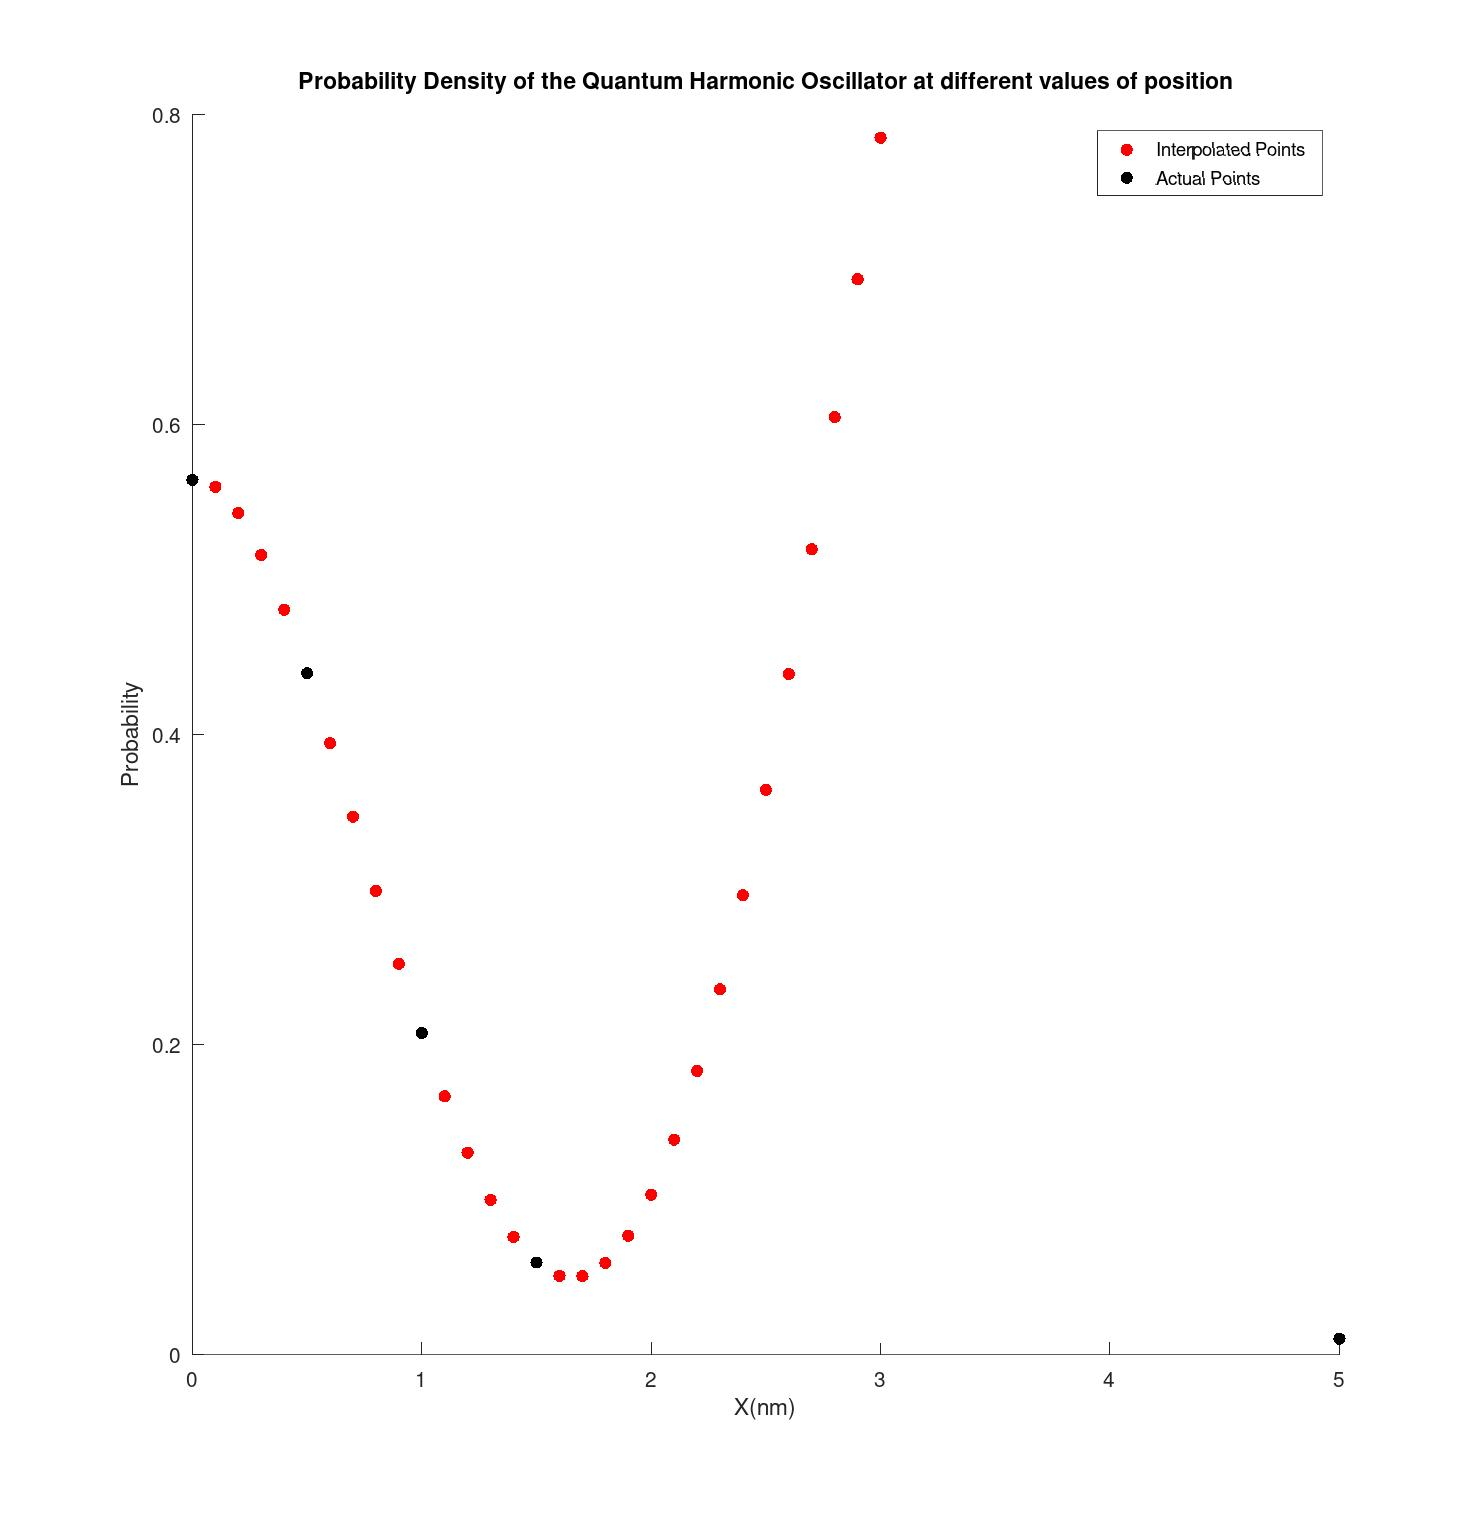
\includegraphics[width=0.75\textwidth]{a4.jpg}
  \caption{Neville’s interpolation of probability density of the quantum harmonic oscillator.}
\end{figure}

\section*{Conclusion}
Neville’s Algorithm was successfully applied to interpolate the probability density
function of the quantum harmonic oscillator. While the method reproduced the general
trend, the observed artifact near the end is a known limitation of polynomial
interpolation. I would like to ask the instructor’s advice on this artifact.
